% vim: set tw=78 sts=2 sw=2 ts=8 aw et ai:
The first step in detecting the above-mentioned attack vector would be to
reliably intercept calls to methods pertaining to Android's cryptographic
framework. Towards this outcome, we will require some of the functionality
exposed by DDI, but with some modifications in order to facilitate preemptive
detection and blocking of malicious applications. Figure \ref{fig:ciphermon}
provides a high-level overview of our proposed solution. We will now outline
each module, as well as their respective interactions.

\begin{figure}[hb]
  \centering
  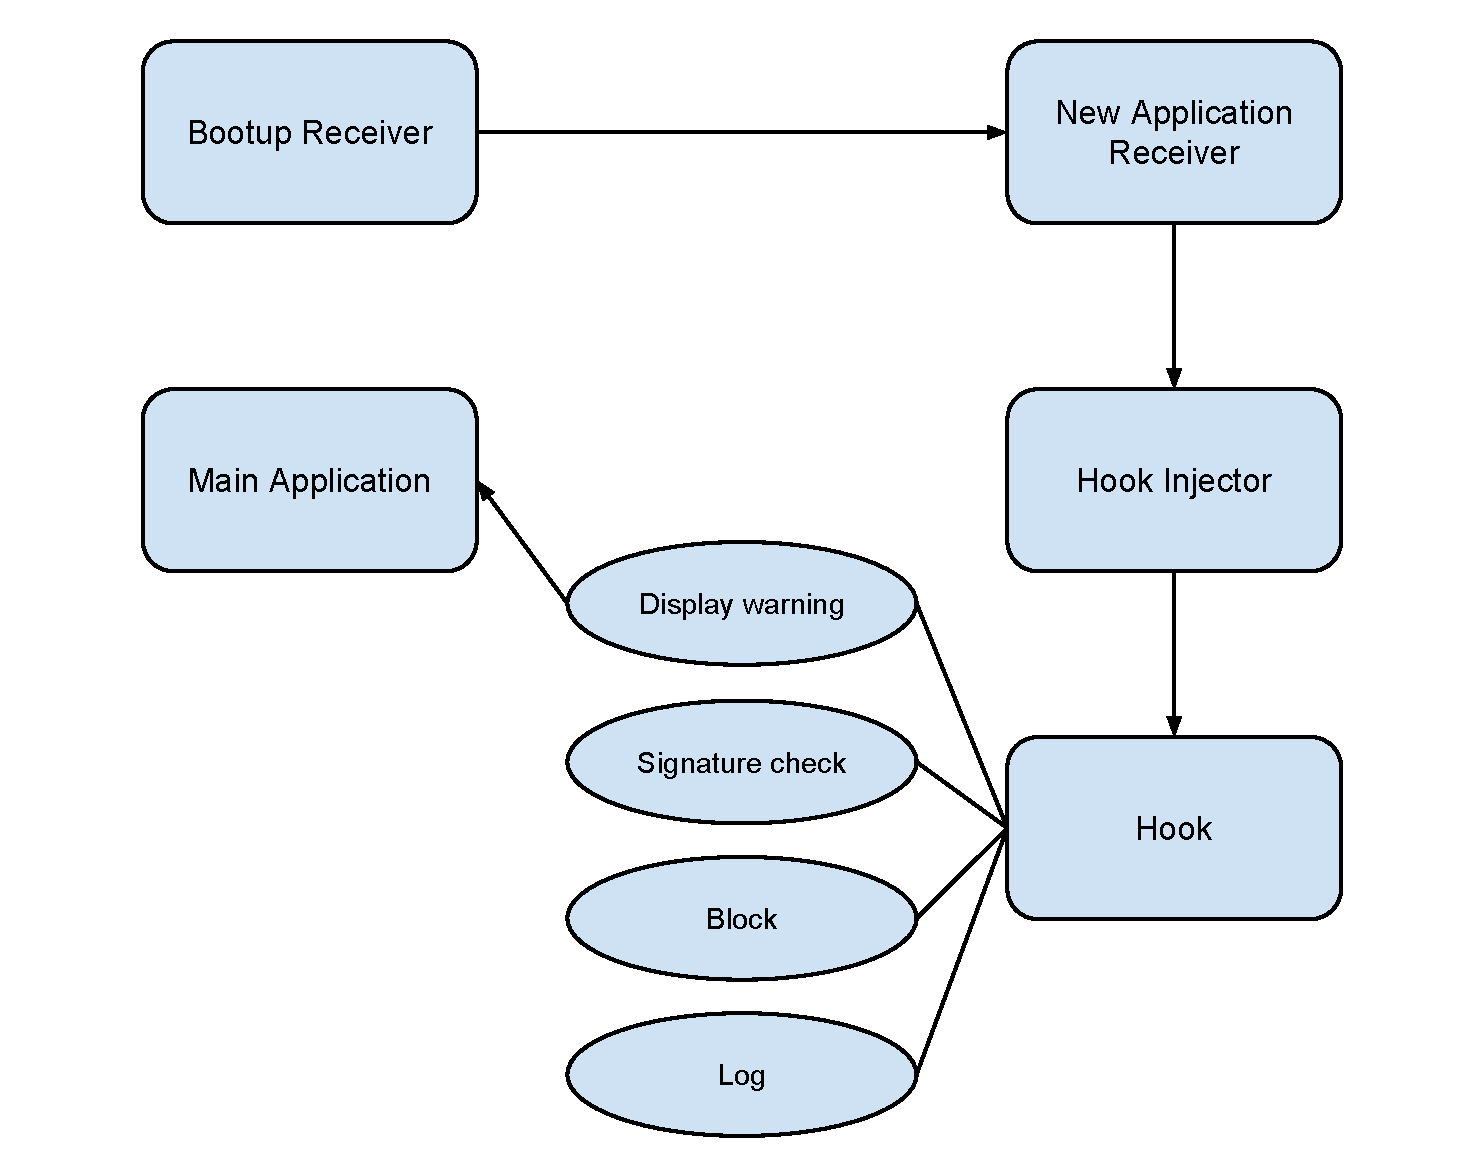
\includegraphics[width=0.5\textwidth]{img/ciphermon}
  \caption{Ciphermon Modules}
  \label{fig:ciphermon}
\end{figure}

\subsection{Bootup Receiver}
We have two prerequisites in order to properly detect malicious applications.
The first is to have a stock Android system, in order to exclude the
possibility that a malicious application is already installed. Such malware
could analyze our solution during installation and take adequate defensive
measures. The second requirement is that the detector start as soon as
possible within the Android booting process. This is mandated since there is
no telling when the user decides to install a new application and our solution
must be already runnning and in active monitoring state.

To this end there is a need for a bootup receiver which waits for a
notification from the Android system that booting has completed. When our
application is notified that the device is ready for normal operation it
enables the New Application Receiver.

\subsection{New Application Receiver}
Since our goal is to block malicious applications from running on the
device, the best angle of approach towards solving this issue would be to
detect when an application is installed. We can leverage the functionality
exposed by the Android framework to detect when a new application is installed
and notify the Hook Injector.

\subsection{Hook Injector}
Whenever a new application is installed, a new thread is spawned that injects
the hook into the memory of Zygote, the Android daemon process that is
responsible for launching new applications. The need for a dedicated thread is
that, in order to inject the hook before the target application is launched, we
must wait for Zygote to create a child process which will load the image of the
target application.

This module is, in fact, an adaptation of the DDI framework and relies heavily
on the work of Collin Mulliner. Since DDI was initially conceived for
security research we had to retrofit it for active runtime detection.

\subsection{Hook}
The hook is a dynamic library that is loaded by the Hook Injector. This is
done by changing the permissions of the code memory area and then writing ARM
assembly that instruments the original function call with our custom wrapper.
Withing this hook we let the original function run and then check the input
and the output buffers using signatures. If both buffers have valid filetype
signatures, we log the malicious attempt, block it from continuing and signal
the Main Application.

\subsection{Main Application}
The Main Application module has a simple purpose, namely to issue a warning to
the user. This notifies the user that there is a suspicious action being carried
out by a certain application.
